\documentclass[english,version-2020-11]{uzl-thesis}


\UzLThesisSetup{
  Masterarbeit,
  Logo-Dateiname        = {uzl-thesis-logo-itcs.pdf},
  Verfasst              = {am}{Institut für Theoretische Informatik},
  Titel auf Deutsch     = {Über elementare Eigenschaften einer mehrdimensionalen Verallgemeinerung des euklidischen Algorithmus},
  Titel auf Englisch    = {On Elementary Properties of a Multi-Dimensional Generalization of the Euclidean Algorithm},
  Autor                 = {Daniel Knaack},
  Betreuerin            = {Prof. Dr. Kim-Manuel Klein},
  Studiengang           = {Informatik},
  Datum                 = {18. Juni 2024},
  Abstract              = {TODO},
  Zusammenfassung       = {TODO},
  Numerische Bibliographie,
}

\UzLStyle{alegrya modern design}

\begin{document}

\chapter{Introduction}

\chapter{Preliminaries}

\section{Generalized Euclidean Algorithm}

\begin{Pseudocode}
while $x$ is not integral do
  solve $Bx = c$
  find $x_l$ which is not integral
  swap $B_l$ and $c$
  ...
end
\end{Pseudocode}

\chapter{Determinant}

\begin{align*}
  x_1     & = 2 - x_2 / x_1 \\
  x_2     & = 2 - x_3 / x_1 \\
  x_3     & = 2 - x_4 / x_1 \\
          & \vdots          \\
  x_{d-1} & = 2 - x_d / x_1 \\
  x_d     & = 1 / x_d - 1   \\
\end{align*}

\begin{itemize}
  \item For odd $d$: $1 - x - 2 x^2 + 2 x^3 - \dots + 2 x^d - x^{d+1} = 0$.
  \item For even $d$: $1 - x - 2 x^2 + 2 x^3 - 2 x^4 \dots - 2 x^d + x^{d+1} = 0$.
\end{itemize}
or in one equation $p_d(x) := 1 - x - (-x)^{d+1} - \sum_{i = 2}^{d} 2 (-x)^{i} = 0$.

\begin{definition}
  Given a polynomial $p = \sum_{i=0}^n a_i x^n$, its reciprocal polynomial,
  denoted as $p^*$, is defined as
  \[
    p^*(x) = x^n p(x^{-1}) = a_n + a_{n-1} x + \dots + a_0 x^n.
  \]
\end{definition}

\begin{example}
  The reciprocal of the previous polynomial $p_d$ is:
  \begin{align*}
    p_d^*(x) & = x^{d+1} - x^d - (-1)^{d+1} + \sum_{i = 2}^{d} -2 (-x)^{d + 1 - i} \\
             & = x^{d+1} - x^d + (-1)^d - \sum_{i = 1}^{d - 1} 2 (-x)^i.
  \end{align*}
\end{example}

\begin{lemma}
  Let $p$ be a polynomial. Then, $a$ is a root of $p$ if and only if $a^{-1}$ is a root of $p^*$.
\end{lemma}

\begin{proof}
  Let $a$ be a root of $p$. It follows $p^*(a^{-1}) = a^n p(a) = a^n \cdot 0 = 0$.
  Now let $a^{-1}$ be a root of $p^*$. Then $p^*(a^{-1}) = a^n p(a) = 0$.
  By construction, $a$ cannot be zero and therefore $p(a) = 0$.
\end{proof}

\begin{definition}
  The characteristic polynomial of a linear recurrence $F$ with coefficients
  $a_0, \dots, a_d$ is defined as
  \[
    p_F(x) = x^{d+1} - \sum_{i = 0}^d a_i x^i.
  \]
\end{definition}

\begin{example}
  The linear recurrence which has $p_d^*(x)$ as its characteristic polynomial is:
  \begin{align*}
    F(n) = F(n - 1) + (-1)^d F(n - d) - \sum_{i=2}^{d - 1} (-1)^{i} 2 F(n - i).
  \end{align*}
\end{example}

% TODO: Show that this converges! We're still missing the convergence criteria
\begin{lemma}
  Let $F$ be a linear recurrence with coefficients $a_0, \dots, a_d$.
  If its characteristic polynomial has a real positive root $\phi$, then
  \[
    \lim_{n \to \infty} \frac{F(n + 1)}{F(n)} = \phi
  \]
\end{lemma}

\begin{proof}
  By the previous lemmas, we can assume that the ratios approach some limit $L$.
  It follows:
  \[
    L
    = \lim_{n \to \infty} \frac{F(n + 1)}{F(n)}
    = \lim_{n \to \infty} a_0 + \sum_{i = 1}^d \frac{a_i F(n - d + i)}{F(n)}
  \]
  Each term in the sum can be rewritten as a product of consecutive terms:
  \[
    \frac{F(n - 1 - d + i)}{F(n - 1)}
    = \frac{F(n - 1 - d + i)}{F(n - d + i)} \frac{F(n - d + i)}{F(n - d + i + 1)} \dots \frac{F(n - 2)}{F(n-1)}.
  \]
  Hence, each term in the sum approaches $L^{-i}$,
  which results in the following polynomial:
  \[
    L = a_0 + \sum_{i = 1}^d a_{d - i} L^{-i},
    \quad \text{or equivalently} \quad
    L^{d+1} = a_0 + a_1 L + \dots + a_d L^d,
  \]
  which directly corresponds to a root of its characteristic polynomial.
\end{proof}

In one dimension, a solution is bad when the value $x_1$ is close to $1$.
However, in the next iteration $x_1$ would be close to $0$ and therefore
would lead to a greater decrease in the determinant.
An initial guess would be that the solution lies exactly between $0$ and $1$ at $1/2$.
However, this solution is also good as after just one step we have achieved integrality.

The solution is to choose a value $x_1$ such that its value in the first
iteration is the same as its value in the second iteration.
This means we are trying to solve the following equation:
\[
  x_1 = 1/x_1 - 1.
\]
This gives us the polynomial $x^2 + x - 1$ where the root is the inverse of the
golden ratio.

% TODO: Explore other strategies. Can we generalize this to every possible strategy?
In just two dimensions, we already have an additional degree of freedom.
Since the solution $x$ consists of two values, we can choose which index we pivot with.
We will choose the value with the smallest fractional value as this decreases
the determinant the fastest.
We assume w.l.o.g. that our values are sorted in increasing order.
This means we pivot with $x_1$ first.

% TODO: What about just choosing the golden ratio for every x_i?
% TODO: Are odd dimensions easier since the decrease is not worse? We could
% choose two values to be the same, since the ratio for odd dimensions is
% smaller than the previous dimension
Just like in one dimension we want to choose $x_1$ carefully such that the
determinant decreases the same amount in every iteration.
A simple solution would be to fill both values with the golden ratio.
In this case, it does not matter which index we choose as each one decreases
the determinant the same amount.
However, in two dimensions we can make this decrease slightly worse
by choosing different values for $x_1$ and $x_2$ such that we swap the pivot
in each iteration.

Assuming the value for $x_1$ is already chosen where would $x_2$ be placed?
Ideally, it would be close to the right side of $x_1$, because then the new
value $-x_2 / x_1$ would be close to $-1$ and the fractional value would be
close to $1$.
Since the decrease must stay the same in each iteration, this gives us the
following two equations:
\begin{align*}
  x_1 = 2 - x_2 / x_1 \\
  x_2 = 1 / x_1 - 1,\\
\end{align*}
which leads to the following polynomial:
\begin{align*}
  x_1^3 - 2x_1^2 - x_1 + 1 = 0
\end{align*}

Let $\phi_2$ be the root of this polynomial.
If we choose $x_1 = \phi_2$ and $x_2 = 2\phi_2 - \phi_2^2$,
then the values in the second iteration are
\[\begin{aligned}
  x_1' & = 1 / x_1 - 1   &  & = 1 / \phi_2 - 1                    &  & = 2\phi_2 + \phi_2^2 &  & = x_2, \\
  x_2' & = 2 - x_2 / x_1 &  & = 2 - (2\phi_2 + \phi_2^2) / \phi_2 &  & = \phi_2             &  & = x_1
\end{aligned}\]

We can extend this to $d$ dimensions using the following equations:
\begin{align*}
  x_1 = 2 - x_2 / x_1 \\
  x_2 = 2 - x_3 / x_1 \\
  x_3 = 2 - x_4 / x_1 \\
  \vdots \\
  x_{d-1} = 2 - x_d / x_1 \\
  x_d = 1 / x_d - 1 \\
\end{align*}

These leads us to two polynomials depending on the dimension.
\begin{itemize}
  \item For even $d$: $x - 1 + 2 x^2 - 2 x^3 + \dots + x^{d+1}$
  \item For odd $d$: $1 - x - 2 x^2 + 2 x^3 - 2 x^4 \dots + x^{d+1}$
\end{itemize}

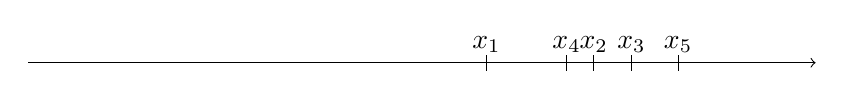
\begin{tikzpicture}[scale=10]
  \draw (0.5820216424559055, -0.01) -- node[above] {$x_1$} (0.5820216424559055, 0.01);
  \draw (0.7181491667223714, -0.01) -- node[above] {$x_2$} (0.7181491667223714, 0.01);
  \draw (0.7661126076135922, -0.01) -- node[above] {$x_3$} (0.7661126076135922, 0.01);
  \draw (0.6837042616132034, -0.01) -- node[above] {$x_4$} (0.6837042616132034, 0.01);
  \draw (0.8252940926247403, -0.01) -- node[above] {$x_5$} (0.8252940926247403, 0.01);
  \draw[->] (0, 0) -- (1, 0);
\end{tikzpicture}

\section{Fibonacci Numbers}

\begin{itemize}
  \item Fibonacci numbers are just linear recurrences with constant coefficients $c_0 = 1, c_1 = 1$.
  \item Linear recurrence with coefficients $c_0, c_1, \dots, c_d$: $a_{n+d+1} = \sum_{i=0}^d c_i a_{n+i}$.
  \item The characteristic polynomial of the Fibonacci sequence is the polynomial of the golden ratio.
  \item For even dimensions: $c_0 = -1, c_1 = 1, c_2 = 2, c_3 = -2, \dots, c_{2d-1} = -2, c_{2d} = 2$.
  \item For odd dimensions:  $c_0 = 1, c_1 = -1, c_2 = -2, c_3 = 2, \dots, c_{2d} = -2, c_{2d+1} = 2$.
  \item The ratio $\phi_d$ for the characteristic polynomials approaches $1/\sqrt{3}$ as $d \to \infty$.
  \item Folding an A4 paper?
\end{itemize}

\chapter{Implementation}

\section{Using an Out-of-the-Box Solver}

\begin{itemize}
  \item Algorithm technically only requires one fractional bit to determine how to round.
  \item Problem: Solving a system of linear equations requires exact fractional solutions.
    Using floating-point numbers leads to inaccurate results.
  \item Could be solved by using an iterative method? However, does a method
    exist, which is accurate up to one fractional bit?
\end{itemize}

\section{Custom Implementation}

\begin{itemize}
  \item Uses custom \texttt{ratio} datatype which implements rational numbers.
  \item Linear system solver implemented using Gaussian elimination and pivoting.
  \item Only the basic algorithm is implemented, so far.
\end{itemize}

\begin{bibtex-entries}
\end{bibtex-entries}

\end{document}
